\section{Convex Hull}
\subsection{Problem Statement}
Implement and compare \textit{Graham Scan} and \textit{Quick Hull} algorithm based on
various input size on randomly generated points.
The comparison metric should be the execution time of each convex hull
finding algorithm.
\subsection{Code}
\begin{code}
    \caption{graham\_scan.cpp}
    \cppcode{../graham_scan.cpp}
    \label{code:graham}
\end{code}

\begin{code}
    \caption{quick\_hull.cpp}
    \cppcode{../quickhull.cpp}
    \label{code:quickhull}
\end{code}

\begin{code}
    \caption{Makefile}
    \begin{minted}{make}
CC=g++

convex: points graham quick

points: generate_points.cpp
	$(CC) $^ -o points.out
	./points.out
graham:	graham_scan.cpp
	$(CC) $^ -o graham_scan.out
	./graham_scan.out

quick: quickhull.cpp
	$(CC) $^ -o quickhull.out
	./quickhull.out

clean:
	rm *.out
    \end{minted}
\end{code}

\subsection{Output}

\begin{figure}[H]
    \centering
    \begin{subfigure}[b]{0.4\textwidth}
        \centering
        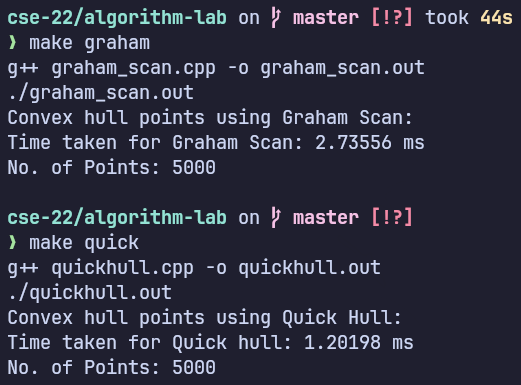
\includegraphics[width=\textwidth]{./img/lab2/p5k.png}
        \caption{Execution time for n=5000}
    \end{subfigure}
    \hfill
    \begin{subfigure}[b]{0.4\textwidth}
        \centering
        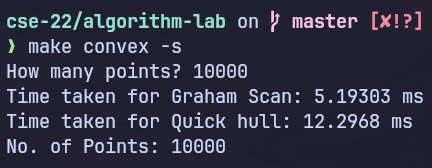
\includegraphics[width=\textwidth]{./img/lab2/p10k.png}
        \caption{Execution time for n=10000}
    \end{subfigure}
    \hfill
    \begin{subfigure}[b]{0.4\textwidth}
        \centering
        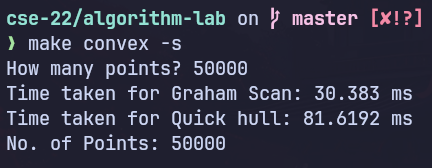
\includegraphics[width=\textwidth]{./img/lab2/p50k.png}
        \caption{Execution time for n=50000}
    \end{subfigure}
    \hfill
    \begin{subfigure}[b]{0.4\textwidth}
        \centering
        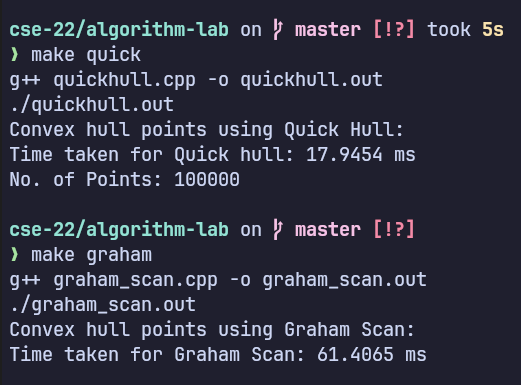
\includegraphics[width=\textwidth]{./img/lab2/p1lack.png}
        \caption{Execution time for n=100000}
    \end{subfigure}
    
    \caption{Convex hull algorithm execution time}
    \label{fig:task1}

\end{figure}

\subsubsection*{Summary of Execution time}

\begin{table}[H]
    \centering
    \caption {Comparison table for Graham Scan \& Quick hull algorithm}
    \label{tab:comp}
\begin{tabular}{lrr}
    \toprule
    \multicolumn{3}{r}{Execution time (ms)} \\
    \cmidrule(c){2-3}
    Input Size & Graham Scan & Quick Hull\\ 
    \midrule
    1000 & 0.460258 & 0.413883\\
    5000 & 2.73556 & 1.20198\\
    10,000 & 5.5254 & 2.73906 \\
    50,000 & 29.7845 & 8.96497 \\
    1,00,000 & 61.4065  & 17.9454 \\
    \bottomrule
\end{tabular}
\end{table}
\subsection{Analysis \& Discussion}
Graham Scan is faster than quick hull for very number of points. 
But with increasing number of points quick hull is significantly efficient
than graham scan. 
This is because Graham scan needs to sort the points before doing its
calculation. And this is more costly. 
In case of quick hull, there is no need to sort the points, rather it can find 
the points by divide and conquer approach, which significantly decreases 
the execution time for quick hull.

\newpage
\section{Matrix Multiplication}
\subsection{Problem Statement}
Implement and compare \textit{Graham Scan} and \textit{Quick Hull} algorithm based on
various input size on randomly generated points.
The comparison metric should be the execution time of each convex hull
finding algorithm.
